\documentclass[a4paper, 11pt]{article}

\usepackage{geometry}
\usepackage{natbib}
\bibpunct[:]{(}{)}{,}{a}{}{;}

%--------------------
%\usepackage{gb4e}
%\noautomath

\usepackage{amsmath}
\usepackage{amsfonts}
\usepackage{amsthm}
\usepackage{amssymb}
\usepackage{mathrsfs}
\usepackage{nicefrac}
%\usepackage{stmaryrd}
%\usepackage{multicol}
\usepackage{graphicx}
\usepackage{color}
\usepackage{booktabs}
\usepackage{pgfplots}
\usepackage{subcaption}
\pgfplotsset{compat=1.3}
\usetikzlibrary{pgfplots.groupplots,decorations.markings}

\newtheoremstyle{Satz}
   {}                      %Space above
   {1em}                   %Space below
   {\normalfont}           %Body font
   {}                      %Indent amount (empty = no indent,
                           %\parindent = para indent)
   {\normalfont}           %Thm head font
   {.}                     %Punctuation after thm head
   {.8em}                  %Space after thm head: " " = normal interword
                           %space; \newline = linebreak
   {\bfseries\thmname{#1}\thmnote{ (#3)}}
                           %Thm head spec (can be left empty, meaning
                           %`normal')

\theoremstyle{Satz}
\newtheorem{example}{Example}

%\newcommand{\mvalueof}[1]{\llbracket#1\rrbracket}
\newcommand{\citeposs}[2][]{\citeauthor{#2}'s (\citeyear[#1]{#2})}
\newcommand{\tuple}[1]{\ensuremath{\left\langle #1 \right\rangle}} 

\newcommand{\hl}[1]{\textcolor[rgb]{.8,.33,.0}{#1}}% prints in orange
%\newcommand{\argmax}[1]{\underset{#1}{\operatorname{arg}\,\operatorname{max}}\;}
%\newcommand{\argmin}[1]{\underset{#1}{\operatorname{arg}\,\operatorname{min}}\;}
%\newcommand{\sbna}{\exists\lnot\forall}

\definecolor{Red}{RGB}{178,34,34}
\newcommand{\mf}[1]{\textcolor{Red}{[MF: #1]}} 
\newcommand{\tb}[1]{\textcolor[rgb]{.8,.33,.0}{[TB: #1]}}% prints in orange

\usepackage{blkarray}
\usepackage{xspace}

\usepackage{tgtermes}
\renewcommand{\baselinestretch}{1.2}

%%% MF's commands
\newcommand{\set}[1]{\left\{#1\right\}}
\newcommand{\card}[1]{\left \lvert \, #1 \, \right\rvert}
\newcommand{\abs}[1]{\lvert #1 \rvert}
\newcommand{\States}{\ensuremath{S}\xspace}		% Set of States
\newcommand{\state}{\ensuremath{s}\xspace}		% single states
\newcommand{\mystate}[1]{\ensuremath{\state_{\text{#1}}}\xspace} %meaningful states
\newcommand{\mylang}[1]{\ensuremath{L_{\text{#1}}}\xspace} %meaningful states
\newcommand{\Messgs}{\ensuremath{M}\xspace}		% Set of Messages
\newcommand{\messg}{\ensuremath{m}\xspace}		% single messages
\newcommand{\mymessg}[1]{\ensuremath{\messg_{\text{#1}}}\xspace} %meaningful messages
\newcommand{\ssome}{\mystate{\ensuremath{\exists\neg\forall}}}
\newcommand{\sall}{\mystate{\ensuremath{\forall}}}
\newcommand{\snone}{\mystate{\ensuremath{\emptyset}}}
\newcommand{\msome}{\mymessg{some}}
\newcommand{\mall}{\mymessg{all}}
\newcommand{\mnone}{\mymessg{none}}
\newcommand{\Lall}{\mylang{all}}
\newcommand{\Lbound}{\mylang{bound}}
\newcommand{\Llack}{\mylang{lack}}
\newcommand{\asome}{\myact{\ensuremath{\exists\neg\forall}}}
\newcommand{\aall}{\myact{\ensuremath{\forall}}}

\definecolor{mygray}{cmyk}{0.35,0.35,0.35,0.35}
\newcommand{\mygray}[1]{{\textcolor{mygray}{#1}}}
%%% 


%--------------------
%
%\usepackage{setspace}
%\onehalfspacing
%
%-------------------


\title{Co-evolution of lexical meaning \& pragmatic use}

\author{%\bf NAME1 and NAME2\\
    ( -- draft \today --- )
}


\date{}

\begin{document}

  %% for arrow head placement
  \tikzset{->-/.style={decoration={
  markings,
  mark=at position #1 with {\arrow{>}}},postaction={decorate}}}
  %%% 

\maketitle

\begin{abstract}
  According to standard linguistic theory, the meaning of an utterance is the product of
  conventional semantic meaning and general pragmatic rules on language use. To investigate how
  cultural evolution of language plays out under this picture of the semantics-pragmatics
  interface, we present a game theoretic model of the competition between types of language
  users, each endowed with a selection of lexical concepts and a particular pragmatic
  disposition to act on them. Our model traces two evolutionary forces and their interaction:
  (i) fitness-based pressure towards communicative efficiency and (ii) potential learning
  biases during the transfer of linguistic knowledge. We illustrate the model based on a case
  study on scalar implicatures. In this case study learning biases that favor simple semantic
  representations can foster the evolution of more sophisticated pragmatic reasoning types and
  so prevent the lexicalization of scalar implicatures.
\end{abstract}

\section{Introduction}\label{sec:introduction}
What is conveyed usually goes beyond what is said. A request for a blanket can be politely
veiled by uttering ``I'm cold;'' temporal succession of events can be communicated by the order
in which conjuncts appear as in ``I traveled to Paris and got married;'' an invitation can be
declined by saying ``I have to work.'' An influential explanation of the relation between the
literal meaning of expressions and what they may convey in context is due to
\citet{grice:1975}, who characterizes pragmatic use and interpretation as a process of mutual
reasoning about rational language use. For instance, under the assumption that the speaker is
cooperative and relevant, ``I have to work'' may be interpreted as providing a reason why the
speaker will not be able to accept an invitation, going beyond its literal meaning. Some of
these enrichments are rather \emph{ad hoc}. Others show striking regularities, such as the use
of ability questions for polite requests (``Could you please \dots?''), or certain enrichments
of lexical meanings such as \emph{and} to convey \emph{and then}.

A particularly productive and well studied class of systematic pragmatic enrichments are scalar
implicatures
\citep{horn:1984,Hirschberg1985:A-Theory-of-Sca,LevinsonPragmatics1983,Geurts2010:Quantity-Implic}. Usually,
the utterance of a sentence like ``I own some of Johnny Cash's albums'' will be taken to mean
that the speaker does not own all of them. This is because, if the speaker instead owned them all, she
could have used the word \emph{all} instead of \emph{some} in his utterance, thereby making a
more informative statement. Scalar implicatures, especially the inference from \emph{some} to
\emph{some but not all}, have been studied extensively, both theoretically
\citep[e.g.,][]{Sauerland2004:Scalar-Implicat,ChierchiaFox2008:The-Grammatical,Rooyvan-RooijJagerde-Jager2012:Explaining-Quan}
as well as experimentally
\citep[e.g.,][]{BottNoveck2004:Some-Utterances,huang+snedeker:2009,GrodnerKlein2010:Some-and-Possib,GoodmanStuhlmuller2013:Knowledge-and-I,DegenTanenhaus2012:Processing-Scal}. While
there is much dispute in this domain about many details, a position endorsed by a clear
majority is that a scalar item like \emph{some} is underspecified to mean \emph{some and maybe
  all} and that the enrichment to \emph{some but not all} is part of some regular process with
roots in pragmatics.

If this majority view is correct, the question arises how such a division of labor between
semantics and pragmatics could have evolved and why it would be so pervasive across natural
languages. Models of language evolution abound. There are simulation-based models studying the
evolution of language in populations of communicating agents
\citep{Hurford1989:Biological-Evol,Steels1995:A-Self-Organizi,LenaertsJansen2005:The-Evolutionar,SteelsBelpaeme2005:Coordinating-Pe,BaronchelliPuglisi2008:Cultural-route-,steels:2011,SpikeStadler2016:Minimal-Require}
and there are mathematical models of language evolution, mostly coming from game theory
\citep{lewis:1969,Warneryd1993:Cheap-Talk-Coor,BlumeKim1993:Evolutionary-St,nowak+krakauer:1999,Huttegger2007:Evolution-and-t,Skyrms2010:Signals}. Much
of this work has focused on explaining basic properties such as compositionality and
combinatoriality
\citep[e.g.,][]{Batali1998:Computational-S,nowak+krakauer:1999,nowak+etal:2000,KirbyHurford2002:The-Emergence-o,kirby:2002,SmithKirby2003:Iterated-Learni,Gong2007:Language-Evolut,kirby+etal:2015,verhoef+etal:2014,Franke2015:Proto-Syntax},
but little attention has been paid to the interaction between conventional meaning and
pragmatic use. What is more, many mathematical models explain evolved meaning as a regularity
in the overt behavior of agents. In contrast, we will here look at language users with a richer
cognitive make-up.


We spell out a model of the co-evolution of conventional meaning and pragmatic reasoning
types. The objects of replication and selection are pairs of lexical meanings and general types
of pragmatic behavior, which we represent using probabilistic models of pragmatic language use
\citep{frank+goodman:2012,FrankeJager2015:Probabilistic-p,GoodmanFrank2016:Pragmatic-Langu}. Replication
and selection are described by the \emph{replicator mutator dynamic}, a general and established
model of evolutionary change in large and homogeneous populations
\citep{Hofbauer1985:The-Selection-M,nowak+etal:2000,NowakKomarova2001:Evolution-of-Un,hofbauer+sigmund:2003,Nowak2006:Evolutionary-Dy}. This
approach allows us to study the interaction between (i) evolutionary pressure towards
communicative efficiency and (ii) possible infidelity in the transmission of linguistic
knowledge, caused by factors such as inductive learning biases and sparse learning
data. Considering transmission of linguistic knowledge is important because neither semantic
meanings nor pragmatic usage patterns are directly observable. Instead, language learners have
to infer these unobservables from the observable behavior in which they result. We formalize
this process as a form of Bayesian inference. Our approach thereby contains a well-understood
model of iterated Bayesian learning \citep{griffiths+kalish:2007} as a special case, but
combines it with functional selection, here formalized as the most versatile dynamic from
evolutionary game theory; the replicator dynamic
\citep{TaylorJonker1978:Evolutionary-St}. Section~\ref{sec:model} introduces this model.

Section~\ref{sec:si-case-study} applies this model to a case study on scalar implicatures. We
discuss a setting in which the majority view of underspecified lexical meanings and pragmatic
enrichments emerges if selection and transmission infidelity are combined. In particular, we
show that inductive learning biases of Bayesian learners that favor simpler lexical meanings
can prevent the lexicalization of scalar inferences and lead to the emergence of Gricean-like
pragmatic reasoning types. Results of this case study are critically assessed in the light of
the assumptions that feed our model in Section~\ref{sec:discussion}.

% We see the main contribution of this work as conceptual and technical, not as a definite answer
% to the question why scalar implicatures emerge. It rather demonstrates how current
% probabilistic cognitive modeling of language use and evolutionary modeling can be fruitfully
% combined to study the co-evolution of semantics and pragmatics side-by-side. Reversely, the
% approach taken here may be seen as a first step towards giving an evolutionary rationale for
% empirically successful probabilistic models of language use that embrace the majority view of
% the division of labor between semantics and pragmatics. Section~\ref{sec:discussion} elaborates
% on these points.

\section{A model of co-evolving lexical concepts and pragmatic behavior}
\label{sec:model}

\subsection{Communicative success and learnability}

The emergence and change of linguistic structure is influenced by many intertwined
factors. These range from biological and socio-ecological to cultural ones \citep{benz+etal:2005b,steels:2011,tamariz+kirby:2016}. Social and ecological pressures determine communicative needs, while
biology determines the architecture that enables and constrains the means by which they can be
fulfilled. In the following, our focus lies on cultural aspects, wherein processes of
linguistic change are viewed as shaped by language use and its transmission, i.e., as a result
of a process of cultural evolution
\citep{Pagel2009:Human-Language-,ThompsonKirby2016:Culture-Shapes-}.

The idea that language is an adaptation to serve a communicative function is fundamental to
many synchronic and diachronic analyses at least since \citeposs{zipf:1949} explanation of word
frequency rankings as a result of competing hearer and speaker preferences \citep[e.g.,
in][]{martinet:1962, horn:1984,jaeger+vRooij:2007,jaeger:2007,
  piantadosi:2014,kirby+etal:2015}. If processes of selection, such as conditional imitation or
reinforcement, favor more communicatively efficient types of behavior, languages are driven
towards semantic expressivity \citep[e.g.,][]{nowak+krakauer:1999,Skyrms2010:Signals}. But
pressure towards communicative efficiency is not the only force that shapes
language. Learnability is another. Natural languages need to be learnable to survive their
faithful transmission across generations. Furthermore, even small learning biases implicit in acquisition
can build up and have quite striking effects on an evolving language in a process of iterated
learning
\citep{KirbyHurford2002:The-Emergence-o,SmithKirby2003:Iterated-Learni,kirby+etal:2014}.

While natural languages are pressured for both communicative success and learnability, these forces may
pull in opposite directions. Their opposition becomes particularly clear when considering the
extreme (cf. \citealt{kemp+regier:2012,kirby+etal:2015}). A language consisting of a single
form-meaning association is easy to learn but lacking in expressivity. Conversely, a language
that lexicalizes a distinct form for a large number of different meanings is highly expressive
but challenging to acquire.

\subsection{The replicator mutator dynamic}

An elegant formal approach to capture the interaction between communicative success and learnability is
the \emph{replicator mutator dynamic}
\citep{Hofbauer1985:The-Selection-M,nowak+etal:2000,NowakKomarova2001:Evolution-of-Un,hofbauer+sigmund:2003,Nowak2006:Evolutionary-Dy}. In
its simplest, discrete-time formulation, the RMD defines the frequency $x'_i$ of each type $i$
in a population at the next time step as a function of: (i) the frequency $x_i$ of each type
$i$ before the update step, (ii) the fitness $f_i$ of each type $i$ before the update, and
(iii) the probability $Q_{ji}$ that an agent who wants to imitate, adopt, or learn the type of
an agent with type $j$ ends up acquiring type $i$:
\begin{align}
  \label{eq:RMD_discrete}
  x'_i = \sum_j Q_{ji} \frac{x_jf_j}{\sum_k x_k f_k}\,.
\end{align}
The RMD consists of two components: fitness-based selection and transmission biases. This
becomes most transparent when we consider an equivalent formulation in terms of a step-wise
application of the discrete-time replicator dynamic \citep{TaylorJonker1978:Evolutionary-St} on the initial population vector $\vec{x}$
and its subsequent multiplication with a mutation matrix $Q$:
\begin{align}
  \label{eq:RMD_discrete_recast}
  x'_i & = (\text{M}(\text{RD}(\vec{x})))_i\,,
\end{align}
where
\begin{align*}
      \left ( \text{RD}(\vec{x}) \right )_i 
         = \frac{x_i f_i}{\sum_k x_k f_k}
 \ \ \ \ \text{and} \ \ \ \ 
  (\text{M}(\vec{x}))_i = (\vec{x} \cdot Q)_i = \left ( \sum_j
          x_j Q_{ji} \right)_i\,.
\end{align*}
If the transmission matrix $Q$ is trivial in the sense that $Q_{ji}=1$ whenever $j=i$, the
dynamic reduces to the replicator dynamic. The replicator dynamic is a model of fitness-based
selection in which the relative frequency of type $i$ will increase with a gradient
proportional to its average fitness in the population. This dynamic is popular and
versatile because it can be derived from many abstract processes of biological and cultural
transmission and selection \citep[for overview and several derivations
see][]{Sandholm2010:Population-Game}, including conditional imitation
\citep[e.g.,][]{Helbing1996:A-Stochastic-Be,Schlag1998:Why-Imitate-and} or reinforcement
learning \citep[e.g.,][]{BorgersSarin997:Learning-Throug,Beggs2005:On-the-Converge}. If fitness
$f_i$ is the same for all types $i$, the replicator step is the identity map
$ \left ( \text{RD}(\vec{x}) \right )_i = x_i$ and the dynamic reduces to a process of
iteration of the transmission bias encoded in $Q$. In this way, the process in
(\ref{eq:RMD_discrete}), equivalently (\ref{eq:RMD_discrete_recast}), contains a model of
iterated learning \citep{griffiths+kalish:2007}. 

\begin{example}
  Consider a simple coordination game. Agents are of two types: positive or negative. If
  agents of different type play with each other, they obtain a payoff of 0. If negative meets
  negative, each receives a payoff of 1. If positive meets positive, they get a payoff of 2. A
  population state is completely characterized by the proportion $x$ of negatives. The fitness
  of negatives in population state $x$ is $f_n(x) = x$, that of positives is $f_p(x) = 2-2x$.
  The average fitness is $\Phi(x) = x f_n(x) + (1-x) f_p(x) = 3x^2 - 4x + 2$. Without mutation,
  the replicator dynamic will then update $x$ to $RD(x) = \nicefrac{x^2}{\Phi(x)}$. The update
  function $RD(x)$ of the replicator step is plotted in Figure~\ref{fig:Updates_RMS} as the
  blue line. Rest points, for which $RD(x)=x$, are at $x=0$, $x=1$ and $x= \nicefrac{2}{3}$.
  The former are attractors as nearby points converge to them. Points near $x=\nicefrac{2}{3}$
  move towards 0 or 1. This is schematically pictured in the topmost phase portrait in
  Figure~\ref{fig:Phase_RD}.

  Adding mutation changes the dynamic and its rest points. Let's assume that $Q_{ji} = .9$
  when $j=i$. The update effect of mutation alone is $M(x) = .9 x + .1 (1-x) = .8x + .1$ and is
  plotted as the linear green line in Figure~\ref{fig:Updates_RMS}. It has only one stable rest
  point at $x = 0.5$ (see Figure~\ref{fig:Phase_RD}). If we first take the replicator step and
  then the mutation step in sequence, we obtain the replicator mutator dynamic
  $RMD(x) = M(RD(x)) = \nicefrac{.9x^2 - .2x +.2}{3x^2 - 4x + 2}$, which is plotted in red in
  Figure~\ref{fig:Updates_RMS}. The rest points are at $x=.121$, $x=.903$ and $x=.609$. The
  former two are attractors (see Figure~\ref{fig:Phase_RD}).
\end{example}



\begin{figure}[t]
  \centering

  %% notice that the figure is hacked, because somehow the curve does not come out right under
  %% PGFplots; I don't know why!?!?
  

    \begin{subfigure}[b]{0.45\textwidth}
      \centering
      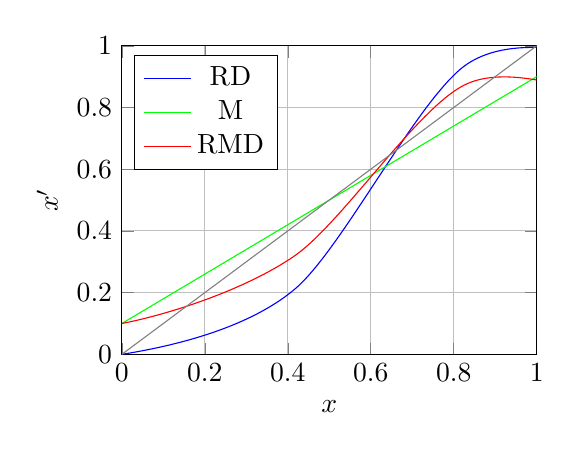
\begin{tikzpicture}
      \begin{axis}[xlabel=$x$, ylabel = $x'$,
                   grid=major, width=6.85cm, height = 5.5cm,
                   legend style = {legend pos = north west},
                   ymin=0,ymax=1, xmin=0,xmax=1]

      \addplot[smooth, color=blue] {x^2 / (3*x^2 - 4*x + 2) + 0.019 * x};
      \addplot[smooth, color=green] {.8*x + .1};

      \addplot[smooth, color=red] {(.9*x^2 - .2*x +.2)/(3*x^2 - 4*x + 2)};

      \addplot[smooth, color=gray] {x};

      \legend{RD, M, RMD}

      \end{axis}
    \end{tikzpicture}


        \caption{Update functions: the population state $x$ is mapped onto $x'$ in one update step}
        \label{fig:Updates_RMS}
    \end{subfigure}
    \hfill
    \begin{subfigure}[b]{0.5\textwidth}    
      \centering
    \begin{tikzpicture}[x=120]
      \node[draw=black, circle, fill = black, minimum size = 0.25cm]
      (0) at (0,0) {};

      \node[draw=black, circle, fill = black, minimum size = 0.25cm]
      (1) at (1,0) {};

      \draw[-, thick] (0) -- (1);

      \node[draw=black, circle, fill = white, minimum size = 0.25cm, thick]
      (mid) at (2/3,0) {};

      \node[]  (0.label) at (0,-0.5) {0};

      \node[]  (1.label) at (1,-0.5) {1};

      \node[]  (label) at (0.5,-0.5) {$x$};

      \node[]  (label) at (0.5,0.55) {RD};

      \draw[->-=0.8,very thick] (mid) -- (0);

      \draw[->-=0.8,very thick] (mid) -- (1);

    \end{tikzpicture}
    
    \vspace*{0.35cm}

    \begin{tikzpicture}[x=120]

      \node (0) at (-0.05,0) {};

      \node (1) at (1.05,0) {};

      \draw[-, thick] (0) -- (1);

      \node[draw=black, circle, fill = black, minimum size = 0.25cm, thick]
      (mid) at (0.5,0) {};

      \node[]  (0.label) at (0,-0.3) {0};

      \node[]  (1.label) at (1,-0.3) {1};

      \node[]  (label) at (0.5,-0.5) {$x$};

      \node[]  (label) at (0.5,0.55) {M};

      \draw[->-=0.5,very thick] (0) -- (mid);

      \draw[->-=0.5,very thick] (1) -- (mid);

    \end{tikzpicture}

    \vspace*{0.35cm}

    \begin{tikzpicture}[x=120]

      \node (0) at (-0.05,0) {};

      \node (1) at (1.05,0) {};

      \node[draw=black, circle, fill = black, minimum size = 0.25cm]
      (S0) at (0.121,0) {};

      \node[draw=black, circle, fill = black, minimum size = 0.25cm]
      (S1) at (0.903,0) {};

      \draw[-, thick] (0) -- (1);

      \node[draw=black, circle, fill = white, minimum size = 0.25cm, thick]
      (mid) at (0.609,0) {};

      \node[]  (0.label) at (0,-0.3) {0};

      \node[]  (1.label) at (1,-0.3) {1};

      \node[]  (label) at (0.5,-0.5) {$x$};

      \node[]  (label) at (0.5,0.55) {RMD};

      \draw[->-=0.5,very thick] (mid) -- (S0);

      \draw[->-=0.5,very thick] (mid) -- (S1);

      \draw[->-=0.5,very thick] (0) -- (S0);

      \draw[->-=0.5,very thick] (1) -- (S1);

    \end{tikzpicture}
        


    \caption{Phase portraits for RD, M and RMD: unstable rest points are hollow, attractors are
      solid.}
        \label{fig:Phase_RD}
    \end{subfigure}

  \caption{Example}
  \label{fig:Example_RMD}
\end{figure}


\subsection{Fitness \& learnability of lexical meanings \& pragmatic strategies}
\label{sec:fitn--learn}

Moving beyond an abstract example, our goal is to apply the RMD to investigate the co-evolution
of lexical concepts and pragmatic behavior. To do so, we need to fix three things: (i) what the
relevant types are, (ii) how fitness derives from communicative success and (iii) how the
mutation matrix $Q$ is computed. These issues are addressed, one by one, in the following.

\subsubsection{Types: Lexica and pragmatic strategies}
\label{sec:languages+use}

Types are what evolution operates on. They define an agent's fitness, usually through a payoff
accrued in single interactions with other agents. Often types can be identified as the possible
acts in a game, e.g., either cooperating or defecting in a prisoner's dilemma. In other cases,
they may be thought of as general properties of an agent that influences her fitness, such as
being positive or negative in our previous example (whatever that means). For our present
purposes, types are identified more concretely by specific assumptions about their cognitive
make-up. Since we are interested in the evolutionary competition between different lexical
concepts and ways of using them in communication, a type is here defined as a pair consisting
of a lexicon and a pragmatic strategy.

Agents play signaling games, in which the speaker wants to communicate a world state $s$ with a
message $m$ to a hearer who receives $m$ but does not know $s$
\citep[e.g.][]{lewis:1969,Skyrms2010:Signals}. A lexicon associates each message with a
(possibly fuzzy) set of states. A pragmatic type maps a lexicon onto a probabilistic speaker
rule (a probabilistic choice of message for each state) and a probabilistic hearer rule (a
probabilistic choice of state for each message). There are many ways of making these general
notions more concrete. Here is what we will assume in the remainder of this paper.

Lexica codify the truth-conditions of expressions. A convenient way to represent lexica is by
$(\card{\States}, \card{\Messgs})$-Boolean matrices, where $\States$ is a set of states
(meanings) and $M$ a set of messages (forms available in the language). For example, suppose
that there are two relevant world states $\States = \set{\ssome, \sall}$. In state $\ssome$
Chris owns some but not all of Johnny Cash's albums while in $\sall$ Chris owns them
all. Suppose that there are two messages $\Messgs = \set{\msome, \mall}$ where $\msome$ is
short for a sentence like \emph{Chris owns some of Johnny Cash's albums} and $\mall$ for the
same sentence with \emph{some} replaced by \emph{all}.  Lexica for this case would assign a
Boolean truth value, either $0$ for false or $1$ for true, to each state-message pair. The
following two lexica are minimal examples for the distinction between a lexicalized upper-bound
for \emph{some} in $\Lbound$ and the widely assumed logical semantics with only a lower-bound
in $\Llack$.

\begin{align*}
  \Lbound & = \begin{blockarray}{lcc}
    & \mygray{\msome} & \mygray{\mall} \\
    \begin{block}{l[cc]}
      \mygray{\ssome} & 1 & 0 \\
      \mygray{\sall}  & 0 & 1 \\
    \end{block}
  \end{blockarray} &
  \Llack & = \begin{blockarray}{lcc}
    & \mygray{\msome} & \mygray{\mall} \\
    \begin{block}{l[cc]}
      \mygray{\ssome} & 1 & 0 \\
      \mygray{\sall}  & 1 & 1 \\
    \end{block}
  \end{blockarray}
\end{align*}

Pragmatic types define dispositions to produce and interpret messages given a lexicon. We
distinguish between two kinds of pragmatic types. {\em Literal interlocutors} produce and
interpret messages literally, being guided only by their lexica. {\em Pragmatic interlocutors}
instead engage in mutual reasoning to inform their choices. Recent probabilistic models of
rational language use
\citep{frank+goodman:2012,FrankeJager2015:Probabilistic-p,GoodmanFrank2016:Pragmatic-Langu}
capture different types of pragmatic behavior in a reasoning hierarchy. The hierarchy's bottom,
level $0$, corresponds to literal language use, as in Equations~(\ref{h:level0}) and
(\ref{s:level0}). Pragmatic language users of level $n + 1$ act (approximately) rational with
respect to level-$n$ behavior of their interlocutors, as in Equations~(\ref{h:leveln}) and
(\ref{s:leveln}).
\begin{alignat}{3}
&H_{0}(s \mid m;L) &&\propto pr(s) L_{sm} \label{h:level0}\\
&S_{0}(m \mid s;L) &&\propto \exp(\lambda \; L_{sm}) \label{s:level0}\\
&H_{n+1}(s|m;L) &&\propto pr(s) S_{n}(m|s;L) \label{h:leveln}\\
&S_{n+1}(m|s;L) &&\propto  \exp(\lambda \; H_{n}(s|m;L)) \label{s:leveln}
\end{alignat}

According to (\ref{h:level0}), a literal hearer's interpretation of a message depends on her
lexicon and her prior over states, $pr \in \Delta(S)$, which is here assumed flat, for
simplicity. Literal interpreters thereby choose an arbitrary true interpretation for each
message. Pragmatic hearers, defined in (\ref{h:leveln}), use Bayes rule to weigh
interpretations based on a conjecture about speaker behavior. Speaker behavior is regulated by
a soft-max parameter $\lambda$, $\lambda \geq 0$ \citep{luce:1959,sutton+barto:1998}. As
$\lambda$ increases, choices approximate strict maximization of expected utilities. Expected
utility of a message $\messg$ in state $\state$ for a level $n+1$ speaker is here defined as
$H_{n}(s|m;L)$, the probability that the hearer will assign to or choose the correct
meaning. For literal speakers, utility only tracks truthfulness. Literal speakers choose any
true message with equal probability but may send false messages as well with a probability
dependent on $\lambda$.

The following examples illustrate these behaviors. A literal interpreter with lexicon $\Lbound$ assigns $\ssome$
a probability of $H_0(\ssome \mid \msome; \Lbound) = 1$ after hearing $\msome$, while a literal
interpreter with $\Llack$ has $H_0(\ssome \mid \msome; \Llack) = 0.5$:
\begin{align*}
  H_0(\cdot \mid \cdot, \Lbound) & = \begin{blockarray}{lcc}
    & \mygray{\ssome} & \mygray{\sall} \\
    \begin{block}{l[cc]}
      \mygray{\msome} & 1 & 0 \\
      \mygray{\mall}  & 0 & 1 \\
    \end{block}
  \end{blockarray} &
  H_0(\cdot \mid \cdot, \Llack) & = \begin{blockarray}{lcc}
    & \mygray{\ssome} & \mygray{\sall} \\
    \begin{block}{l[cc]}
      \mygray{\msome} & .5 & .5 \\
      \mygray{\mall}  & 0 & 1 \\
    \end{block}
  \end{blockarray} 
\end{align*}
If $\lambda = 1$ literal speaker behavior looks like this:
\begin{align*}
  S_0(\cdot \mid \cdot, \Lbound) & \approx \begin{blockarray}{lcc}
    & \mygray{\msome} & \mygray{\mall} \\
    \begin{block}{l[cc]}
      \mygray{\ssome} & .73 & .27 \\
      \mygray{\sall}  & .27 & .73 \\
    \end{block}
  \end{blockarray} &
  S_0(\cdot \mid \cdot, \Llack) & \approx \begin{blockarray}{lcc}
    & \mygray{\msome} & \mygray{\mall} \\
    \begin{block}{l[cc]}
      \mygray{\ssome} & .73 & .27 \\
      \mygray{\sall}  & .5 & .5 \\
    \end{block}
  \end{blockarray} 
\end{align*}
If $\lambda = 20$, literal speakers will choose true utterances with less slack:
\begin{align*}
  S_0(\cdot \mid \cdot, \Lbound) & \approx \begin{blockarray}{lcc}
    & \mygray{\msome} & \mygray{\mall} \\
    \begin{block}{l[cc]}
      \mygray{\ssome} & 1 & 0 \\
      \mygray{\sall}  & 0 & 1 \\
    \end{block}
  \end{blockarray} &
  S_0(\cdot \mid \cdot, \Llack) & \approx \begin{blockarray}{lcc}
    & \mygray{\msome} & \mygray{\mall} \\
    \begin{block}{l[cc]}
      \mygray{\ssome} &  1 & 0 \\
      \mygray{\sall}  & .5 & .5 \\
    \end{block}
  \end{blockarray} 
\end{align*}
Pragmatic hearers of level 1 have the following probabilistic interpretation behavior for
$\lambda = 1$:
\begin{align*}
  H_1(\cdot \mid \cdot, \Lbound) & \approx \begin{blockarray}{lcc}
    & \mygray{\ssome} & \mygray{\sall} \\
    \begin{block}{l[cc]}
      \mygray{\msome} & .73 & .27 \\
      \mygray{\mall}  & .27 & .73 \\
    \end{block}
  \end{blockarray} &
  H_1(\cdot \mid \cdot, \Llack) & \approx \begin{blockarray}{lcc}
    & \mygray{\ssome} & \mygray{\sall} \\
    \begin{block}{l[cc]}
      \mygray{\msome} & .59 & .41 \\
      \mygray{\mall}  & 0.35 & 0.65 \\
    \end{block}
  \end{blockarray} 
\end{align*}
For $\lambda = 20$, there will less slack again:
\begin{align*}
  H_1(\cdot \mid \cdot, \Lbound) & \approx \begin{blockarray}{lcc}
    & \mygray{\ssome} & \mygray{\sall} \\
    \begin{block}{l[cc]}
      \mygray{\msome} & 1 & 0 \\
      \mygray{\mall}  & 0 & 1 \\
    \end{block}
  \end{blockarray} &
  H_1(\cdot \mid \cdot, \Llack) & \approx \begin{blockarray}{lcc}
    & \mygray{\ssome} & \mygray{\sall} \\
    \begin{block}{l[cc]}
      \mygray{\msome} & 0.67 & 0.33 \\
      \mygray{\mall}  & 0 & 1 \\
    \end{block}
  \end{blockarray} 
\end{align*}
With $\lambda = 1$, pragmatic speakers of level 1 will have:
\begin{align*}
  S_1(\cdot \mid \cdot, \Lbound) & \approx \begin{blockarray}{lcc}
    & \mygray{\msome} & \mygray{\mall} \\
    \begin{block}{l[cc]}
      \mygray{\ssome} & .73 & .27 \\
      \mygray{\sall}  & .27 & .73 \\
    \end{block}
  \end{blockarray} &
  S_1(\cdot \mid \cdot, \Llack) & \approx \begin{blockarray}{lcc}
    & \mygray{\msome} & \mygray{\mall} \\
    \begin{block}{l[cc]}
      \mygray{\ssome} & .62 & .38 \\
      \mygray{\sall}  & .38 & .62 \\
    \end{block}
  \end{blockarray} 
\end{align*}
For high $\lambda = 20$, pragmatic speakers of level 1 give us:
\begin{align*}
  S_1(\cdot \mid \cdot, \Lbound) & \approx \begin{blockarray}{lcc}
    & \mygray{\msome} & \mygray{\mall} \\
    \begin{block}{l[cc]}
      \mygray{\ssome} & 1 & 0 \\
      \mygray{\sall}  & 0 & 1 \\
    \end{block}
  \end{blockarray} &
  S_1(\cdot \mid \cdot, \Llack) & \approx \begin{blockarray}{lcc}
    & \mygray{\msome} & \mygray{\mall} \\
    \begin{block}{l[cc]}
      \mygray{\ssome} & 1 & 0 \\
      \mygray{\sall}  & 0 & 1 \\
    \end{block}
  \end{blockarray} 
\end{align*}

It is important to note that pragmatic agents of level 1 using $\Llack$ associate $\msome$
preferentially with $\ssome$, in contrast to their literal counterparts of level 0. This
association is not perfect, and usually less strong than what agents with a lexicalized upper
bound in $\Lbound$ can achieve, even without pragmatic reasoning. Higher order 
reasoning types leads to stronger associations of $\msome$ and $\ssome$ also for the
hearer. Still, the case study presented in Section~\ref{sec:si-case-study} will consider
speaker and hearer behavior at levels 0 and 1, as the latter are the simplest pragmatic
reasoning types which show a tendency to communicatively attuned pragmatic enrichment. Using
only level 1 reasoning types is therefore a conservative choice that works against the
fitness-based selection of pragmatic language use for a notion of fitness based on
communicative efficiency, which is introduced next.

\subsubsection{Fitness \& fitness-based selection based on communicative success}\label{sec:expressivity}

Under the replicator dynamic the proportion of type $i$ in a population will increase or
decrease as a function of its relative fitness $f_i$. In the context of language evolution,
fitness is usually associated with the ability to successfully communicate
with other language users from the same population
\citep[e.g.,][]{nowak+krakauer:1999,nowak+etal:2000, nowak+etal:2002}. Under a biological
interpretation the assumption is that organisms have a higher chance of survival and
reproduction if they are able to share and receive useful information via communication with
peers. Under a cultural interpretation the picture is that agents themselves strive towards
communicative success and therefore occasionally adapt or revise their behavior to achieve
higher communicative success (see \citealt[\S3.3]{benz+etal:2005b} for discussion).

The replicator equation gives us the means to make the ensuing dynamic precise, without
necessarily committing to a biological or cultural interpretation. As above, the proportion of
types in a given population is codified in a vector $\vec{x}$, where $x_i$ is the proportion of
type $i$. The fitness of type $i$ is its average expected communicative success, or
\emph{expected utility} (EU), given the frequencies of types in the current population:
\begin{align*}
  f_i = \sum_j x_j \text{EU}(t_i,t_j)\,.
\end{align*}
In signaling games, the expected utility $\text{EU}(t_i,t_j)$ for type $i$ when communicating with type $j$ is the
average success of $i$ when talking or listening to $j$. If agents are speakers half of the
time, this yields:
\begin{align*}
  \text{EU}(t_i,t_j) = \nicefrac{1}{2} \, \text{EU}_S(t_i,t_j) + \nicefrac{1}{2} \, \text{EU}_H(t_i,t_j)\,,
\end{align*}
where $\text{EU}_S(t_i,t_j)$ and $\text{EU}_H(t_i,t_j)$ are the expected utilities for $i$ as a
speaker and as a hearer when communicating with $j$, defined as follows, where $n_i$ and $n_j$
are type $i$'s and type $j$'s pragmatic reasoning types and $L_i$ and $L_j$ are their lexica:
\begin{flalign*}
  & \text{EU}_S(t_i,t_j)  = \sum_s P(s)\sum_m S_{n_i}(m \mid s;L_i) \sum_{s'} H_{n_j}(s' \mid m;L_j)
  \delta(s,s') \,, \\
 & \text{EU}_H(t_i,t_j)  = \text{EU}_S(t_j,t_i)\,.
\end{flalign*}
As usual, $\delta(s,s') = 1$ iff $s = s'$ and $0$ otherwise.

\subsubsection{Learnability}
\label{sec:learnability}

Languages are shaped not only by functionalist forces towards greater communicative success. Another
important factor is the fidelity with which linguistic knowledge is transmitted. Among others,
linguistic production can be prone to errors, states or messages may be perceived incorrectly,
and multiple languages may be compatible with the data learners are exposed to. These sources
of uncertainty introduce variation in the transmission of linguistic knowledge from one
generation to the next. In particular, learning biases in the iterated transmission process can
influence language evolution substantially.

In biological evolution, where types are expressed genetically, transmission infidelity comes
into the picture through infrequent and mostly random genetic mutations. However, an agent's
lexicon and pragmatic reasoning behavior is likely not inherited genetically. They need to be
learned from observation. Concretely, when agents of type $j$ want to adopt or imitate the
linguistic behavior of type $i$, they observe the overt linguistic behavior of type $i$ and
need to infer the covert type that most likely produced the visible behavior. Iterated learning
is a process in which languages are learned repeatedly from the observation of linguistic
behavior of agents who have themselves acquired the language from observation and inference. In
the simplest case there is a single teacher and a single learner. After sufficient training the
learner becomes a teacher and produces behavior that serves as input for a new learner. Due to
the pressure towards learnability it exerts, iterated learning alone generally leads to simpler
and more regular languages (see \citealt{kirby+etal:2014} and \citealt{tamariz+kirby:2016} for
recent surveys).

Following \citet{griffiths+kalish:2007} we model language acquisition as a process of Bayesian
inference in which learners combine the likelihood of a type producing the witnessed learning
input with prior inductive biases. Experimental and mathematical results on iterated learning
suggest that the outcome of this process reflects learners' inductive biases
\citep[e.g.,][]{kirby+etal:2014}. In a Bayesian setting these biases can be codified in a prior
$P \in \Delta(T)$, which reflects the amount of data a learner requires to faithfully acquire
the language of the teacher \citep[cf.][450]{griffiths+kalish:2007}. The extent of the prior's
influence has been shown to heavily depend on the learning strategy assumed to underlie the
inference process. On the one hand, early simulation results suggested that weak biases could
be magnified by exposing learners to only small data samples
\citep[e.g. in][]{brighton:2002}. On the other, \citeposs{griffiths+kalish:2007} mathematical
characterization showed that iterated learning converges to the prior in the limit, i.e., that
the resulting distribution over languages corresponds to the learners' prior distribution and
is not influenced by the amount of input given to them. This difference in predictions can be
traced back to differences in the selection of hypotheses from the posterior. Griffith \&
Kalish's convergence to the prior holds for learners that sample from the posterior. More
deterministic strategies such as the adoption of the type with the highest posterior
probability, so-called {\it maximum a posterior estimation} (MAP), increase the influence of
both the prior and the data \citep{griffiths+kalish:2007,kirby+etal:2007}. In the following, we
use a parameter $l\ge1$ to modulate between posterior sampling and the MAP strategy. When
$l = 1$ learners sample from the posterior. The learners' propensity to maximize the posterior
grows as $l$ increases.

Let $D$ be the set of possible data that learners may be exposed to. This set $D$ contains all
sequences of state-message pairs of length $k$, e.g.,
$\tuple{\tuple{s_1,m_1},\dots , \tuple{s_k,m_k}}$. As $k$ increases, learners have more data to base their inference on and so tend to
recover the true types that generated a given sequence with higher probability. The mutation
matrix $Q$ of the replicator mutator dynamic in (\ref{eq:RMD_discrete}) can then be defined as
follows: $Q_{ji}$ is the probability that a learner acquires type $i$ when learning from an
agent of type $j$. The learner observes a length-$k$ sequence $d$ of state-message pairs, but
the probability $P(d \mid t_j)$ with which sequence $d = \tuple{\tuple{s_1,m_1},\dots , \tuple{s_k,m_k}}$ is observed depends on type $j$'s
behavior:
\begin{align*}
  P(d = \tuple{\tuple{s_1,m_1},\dots , \tuple{s_k,m_k}} \mid t_j) = \prod_{i = 1}^k S_{n_j}(m_i
  \mid s_i; L_{j})\,,
\end{align*}
where, as before, $n_j$ is $j$'s pragmatic reasoning type and $L_j$ is $j$'s lexicon. For a
given observation $d$, the probability of acquiring type $i$ is $F(t_i \mid d)$, so that:
\begin{flalign*}
  Q_{ji} \propto \sum_{d \in D} P(d \mid t_j) F(t_i \mid d)\,.
\end{flalign*}
The acquisition probability $F(t_i \mid
d)$ given datum $d$ is obtained by probability matching $l = 1$ or a tendency towards choosing
the most likely type $l > 1$ from the posterior distribution $P(\cdot \mid d)$ over types given
the data, which is calculated by Bayes' rule:
\begin{flalign*}
  & F(t_i \mid d) \propto P(t_i \mid d)^l \; \text{ and }\\
  & P(t_i \mid d) \propto P(t_i) P(d \mid t_i)\,.
\end{flalign*}


\subsection{Model summary}

Communicative success and learnability are central to the cultural evolution of language. These
components can be modelled, respectively, as replication based on a measure of fitness in terms
of communicative efficiency and iterated Bayesian learning. Their interaction is described by
the discrete time replicator mutator dynamic in (\ref{eq:RMD_discrete}), repeated here:
\begin{align*}
  x'_i = \sum_j Q_{ji} \frac{x_jf_j}{\sum_k x_k f_k}\,.
\end{align*}
This equation defines the frequency $x'_i$ of type $i$ at the next time step, based on its
frequency $x_i$ before the step, its fitness $f_i$, and the probability that a learner infers
$i$ when observing the behavior of a type-$j$ agent. Fitness-based selection is here thought of
not as biological (fitness as expected relative number of offspring) but cultural (fitness as
likelihood of being imitated or repeated) evolution, since the types that the dynamic operates
on are pairs consisting of a lexicon and a pragmatic use pattern. A type's communicative success depends
on how well it communicates within a population while its learnability depends on the
fidelity by which it is inferred by new generations of learners. The learners' task is
consequently to perform a joint inference over types of linguistic behavior and lexical
meaning.

The model has three parameters: $\lambda$ regulates the degree to which pragmatic speakers
choose messages that maximize the chance of communicative success; $k$ is the number of
observations for each language learner; $l$ regulates where the learners' inference behavior
lies on a spectrum from probability matching to choice of the most likely parent type.


\section{Case study: scalar implicatures}
\label{sec:si-case-study}

The model of the previous section formalizes the evolutionary competition between different
pairs of lexical concepts and ways of using them. This section looks at a case study on scalar
implicatures. It engages in a following formal thought experiment to address the question: if a
population of language users could freely combine different lexica with different pragmatic
strategies, what are conditions under which the majority view of scalar implicatures could have
evolved?

Recall that the majority view is that scalar implicatures are non-lexicalized pragmatic
enrichments. Scalar implicature triggers like \emph{some}, \emph{warm} or \emph{may} are
semantically weak expressions for which logically stronger expressions are salient, e.g.,
\emph{all}, \emph{hot} or \emph{must}. For instance, {\em some} is entailed by {\em all}. If
the sentence ``Chris owns all of Johnny Cash's albums'' is true, then ``Chris owns some of
Johnny Cash's albums'' is also true. However, while weaker expressions such as {\em some} are
truth-conditionally compatible with stronger alternatives such as {\em all}, this is not what
their use is normally taken to convey. Instead, the use of a less informative expression when a
more informative one could have been used can license a defeasible inference that stronger
alternatives do not hold (cf. \citealt{horn:1972,gazdar:1979}). In this way, ``Chris owns some
of Johnny Cash's albums'' is strengthened to convey that she owns {\em some but not all}
albums. According to the majority view, this is a pragmatic inference, not part of the
conventional meaning.

In the following we consider a specific application of the model from Section~\ref{sec:model}
which allows to address the question if or when scalar inferences might (not) lexicalize. We
consider what is perhaps one of the simplest non-trivial setups that speak to this matter and
reflect on its limitations in Section~\ref{sec:discussion}. The setup is introduced in
Section~\ref{sec:setup:-stat-conc}. Section~\ref{sec:simulation-results} describes the simulations
and their results.

% Our initial question about the division of labor between semantics and pragmatics can be narrowed to the case of scalar implicatures by asking for a justification for the lack of lexical upper-bounds in weak scalar alternatives. That is, we ask why lexical meanings that lack upper-bounds and convey it pragmatically are regularly selected for over alternatives such as that of codifying the bound semantically. More poignantly, would it not serve language users better if weak(er) expressions such as {\em warm}, {\em or}, {\em some} and {\em big} were truth-conditionally incompatible with stronger alternatives such as {\em hot}, {\em and}, {\em all} and {\em huge} to avoid misunderstanding?  This question is particularly striking considering the number of expressions that license such inferences across natural languages. 


\subsection{Setup}
\label{sec:setup:-stat-conc}

To fill the model from Section~\ref{sec:model} with life, we need to specify the sets of
states, messages and lexica (Section~\ref{sec:stat-mess-conc}). Additionally, we want to
explore the effects of a learning bias in favor of simple lexical concepts. One way of
motivating and formalizing such a bias is introduced below in
Section~\ref{sec:an-induct-learn}.


\subsubsection{States, messages, concepts and lexica} 
\label{sec:stat-mess-conc}

Consider a state space with three states $\States = \set{\snone, \ssome, \sall}$ and think of
it as a partition of possible worlds into cells where none, some or all of the $A$s are $B$s,
for some arbitrary fixed predicates $A$ and $B$. Eight concepts can be distinguished based on
their truth or falsity in three world states, six of which are not contradictory or
tautological (see Table~\ref{tab:concepts} below).

A lexicon $L$ is a mapping $\Messgs \rightarrow C$ from messages to concepts. With three
messages there are $6^3 = 216$ possible lexica. Some assign the same concept to more than one
message and others lexicalize the same concepts but associate them with different messages. Out
of these possible lexica, three kinds are of particular relevance. First, lexica that assign
the same concept to more than one message. Such lexica lack in expressivity but may be favored
by particular learning biases nonetheless (see below). Second, lexica that conventionalize
upper-bounds to realize a one-to-one mapping of messages to states. Finally, lexically that do
not lexicalize an upper bound but allow it to be conveyed pragmatically due to the presence of
a stronger lexical item. There are six lexica of the second kind and six of the third. The
following three lexica exemplify each kind:
\begin{align*}
  \begin{blockarray}{lccc}
    & & \underline{\Lall} & \\
    & \mygray{\mnone} & \mygray{\msome} & \mygray{\mall} \\
    \begin{block}{l[ccc]}
     \mygray{\snone}  & 0 & 0 & 0\\
     \mygray{\ssome}  & 0 & 0 & 0\\
    \mygray{\sall}   & 1 & 1 & 1\\
    \end{block}
% \\ & & P(\Lall)\rlap{ $\propto 9$} & \\
  \end{blockarray} & &
 \begin{blockarray}{lccc}
    & & \underline{\Lbound} & \\
    & \mygray{\mnone} & \mygray{\msome} & \mygray{\mall} \\
    \begin{block}{l[ccc]}
       & 1 & 0 & 0\\
       & 0 & 1 & 0\\
       & 0 & 0 & 1\\
    \end{block}
%  \\& & P(\Lbound)\rlap{ $\propto 96$} & \\
  \end{blockarray} & &
  \begin{blockarray}{lccc}
    & & \underline{\Llack} & \\
    & \mygray{\mnone} & \mygray{\msome} & \mygray{\mall} \\
    \begin{block}{l[ccc]}
       & 1 & 0 & 0\\
       & 0 & 1 & 0\\
       & 0 & 1 & 1\\
    \end{block}
%   \\& & P(\Llack)\rlap{ $\propto 48$} & \\
  \end{blockarray}
\end{align*}
Lexicon $\Lall$ is clearly bad for communication: all message and interpretation choices will
be equally likely for all types; no information about the observed world state will be conveyed
by its users. In contrast, users of $\Lbound$ can communicate world states perfectly, no matter
whether they are literal or pragmatic users. Users of $\Llack$ can also communicate information
about the actual world state but need pragmatic language use to approximate a one-to-one
mapping between message use and states (see Section~\ref{sec:languages+use}).

Recall that types are a combination of a lexicon and a manner of language use. We analyze the
model's predictions in populations of types with one of the two behaviors introduced earlier;
literal or pragmatic. The former correspond to level $0$ reasoners and the latter to level
$1$. Accordingly, we consider a total of $432$ types. Six are variants of pragmatic language
users with $\Llack$-like lexica. We refer to these as \emph{target types}, because they
represent lexica and language use that conform to the majority view of scalar
implicatures. Twelve types are either literal or pragmatic speakers with lexical of the
$\Lbound$ kind. We refer to these as \emph{competitor types}, because they are expected to be
the target types' main competitors in evolutionary competition.



\subsubsection{An inductive learning bias for semantic simplicity}
\label{sec:an-induct-learn}

There is a growing effort to develop empirically testable representational languages that allow
for the measure of semantic complexity. For instance, so-called {\em languages of thought}
(LOTs) have been put to test in various rational probabilistic models that show encouraging
results (see, e.g., \citealt{katz+etal:2008, piantadosi+etal:underreview,
  piantadosi+etal:2012a} and \citealt{piantadosi+jacobs:2016} for recent discussion). At its
core, a LOT defines a set of operations and composition rules from which concepts can be
derived. As a first approximation and for the sake of concreteness, we follow this approach to
motivate and formalize a preference of learners for simpler semantic representations
(\citealt{feldman:2000, chater+vitanyi:2003, piantadosi+etal:2012a,kirby+etal:2015}, \citeauthor{piantadosi+etal:underreview} under review). A concept's complexity is a function of its
derivation cost in a weighed generative LOT.

\begin{table}
  \centering
  \begin{align*}
    C & \rightarrow_2 C \wedge C 
    & C & \rightarrow_2 \neg C  \\ 
    C & \rightarrow_1 X \subseteq X &
    C & \rightarrow_1 X \neq \emptyset &
    C & \rightarrow_1 X = \emptyset  \\
    X & \rightarrow_1 \set{A,B} & 
    X & \rightarrow_1 X \cap X & 
    X & \rightarrow_1 X \cup X    
  \end{align*}
  \caption{Toy grammar in a set-theoretic LOT with weighted rules.}
  \label{tab:grammar}
\end{table}

Our toy grammar of concepts is given in Table~\ref{tab:grammar}. This grammar uses basic
set-theoretic operations to form expressions which can be evaluated as true or false in states
$\snone$, $\ssome$ or $\sall$ from above. Applications of generative rules have a cost attached
to them. Here we simply assume that the formation of Boolean combinations of concepts incurs 2
cost units, while all other rule applications incur only 1 cost unit. Table~\ref{tab:concepts}
lists all six concepts relevant here, their truth conditions and the simplest formula that
expresses this concept from the grammar in Table~\ref{tab:grammar}.

\begin{table}
  \centering
\begin{center}
  \begin{tabular}{lccclc}
    \toprule
    intuitive name
    & \snone
    & \ssome
    & \sall
    & least complex formula
    & complexity
    \\ \midrule
    ``all''
    & 0
    & 0
    & 1
    & $A \subseteq B$
    & $3$
    \\
    ``some but not all''
    & 0
    & 1
    & 0
    & $A \cap B \neq \emptyset \wedge A \neq \emptyset$
    & $8$
    \\    
    ``some''
    & 0
    & 1
    & 1
    & $A \cap B \neq \emptyset$
    & $4$
    \\
    ``none''
    & 1
    & 0
    & 0
    & $A \cap B = \emptyset$
    & $4$
    \\
    ``none or all''
    & 1
    & 0
    & 1
    & $\neg(A \cap B \neq \emptyset \wedge A \neq \emptyset)$
    & $10$
    \\
    ``not all''
    & 1
    & 1
    & 0
    & $\neg (A \subseteq B)$
    & $5$
    \\
    \bottomrule
  \end{tabular}
\end{center}
\caption{Available concepts and their minimal derivation cost}
\label{tab:concepts}
\end{table}

The complexity measure for lexical concepts from Table~\ref{tab:concepts} is used to define a
learning bias that favors simpler concepts over more complex ones. The prior probability of a
type is just the prior probability of its lexicon. The prior of a lexicon is a function of the
complexity of the lexical representations in its image set. Lexica with simpler concepts have a
higher prior. One simple way of defining such priors over lexica (and thereby types) is:
\begin{align*}
  P(L)  & \propto \prod_{c \in Im(L)} P(c)   \ \text{, with} & 
  P(c) & \propto \max_{c'}Compl(c') - Compl(c) + 1\,,
\end{align*}
where $Compl(c)$ is the complexity of the minimal derivation cost of $c$ according to the
LOT-grammar (see Table~\ref{tab:concepts}). Applied to our space of lexica, this construal assigns the highest probability 
to a lexicon of type $\Lall$, which only uses the simplest concept ``all'' for
all messages. Lexica of type $\Llack$ are less likely, but more likely than $\Lbound$. 

There are many ways to define priors over lexica (see, e.g., \citealt{goodman+etal:2008,
  piantadosi+etal:2012a}) but the key assumption here, common to all of them, is that simple
representational expressions should be favored over more complex ones. We should stress that
these details -- from the generative grammar to its complexity measure -- are to be regarded as
one convenient operationalization of one general approach to explicating learning biases; this
is not a commitment that this general approach is necessarily superior or that, within it, this
particular instrumentalization is the single most plausible.


\subsection{Simulation results}
\label{sec:simulation-results}

Recall that there are three parameters: soft-max parameter $\lambda$ affects how strongly
speakers favor messages that appear best from their subjective point of view; the
bottleneck size $k$ influences how faithfully learners can identify their teacher type; $l$
defines the learners' disposition towards choosing the most likely teacher type from the
posterior distribution. We expect that competitor types (types with lexica of the kind
$\Lbound$) have a fitness advantage over target types (pragmatic agents with lexica of the kind
$\Llack$), especially for very low levels of $\lambda$. Selection based on fitness alone may
therefore not lead to prevalence of target types in the population. On the other hand, lexica
of type $\Llack$ are simpler than those of type $\Lbound$ by the postulated measure from
above. This may make them more likely to be adopted by learners, especially when $k$ is low so
that different teacher types are relatively indistinguishable based on their behavior and when
$l$ is high. Still, lexica of the kind $\Lall$ are in turn more likely \emph{a priori} than
lexica of the kind $\Llack$. Simulation results will shed light on the question whether target
types can emerge and for which parameter constellations.

To better understand the workings of a pressure towards communicative efficiency and a pressure
towards learnability, we look at the behavior of the replicator and mutator step first in
isolation, and then in combination. All simulation runs are initialized with an arbitrary
distribution over types, constituting a population's first generation. All reported results are
the outcome of 50 update steps. These outcomes correspond to developmental plateaus in which
change is, if not absent, then at least very slow. In other words, even if the resulting states
do not correspond to an eventual attracting state, they characterize long almost stationary
states in which the system remains for a very long time. As specified in
\S\ref{sec:learnability}, the mutation matrix $Q$ can be obtained by considering all possible
state-message sequences of length $k$. Given that this is intractable for large $k$, the sets
of data learners are exposed to are approximated by sampling $250$ $k$-length sequences from
each type's production probabilities.


\subsubsection{Replication only: selection based on expressivity and communicative success} 


\begin{figure}[t]
\centering
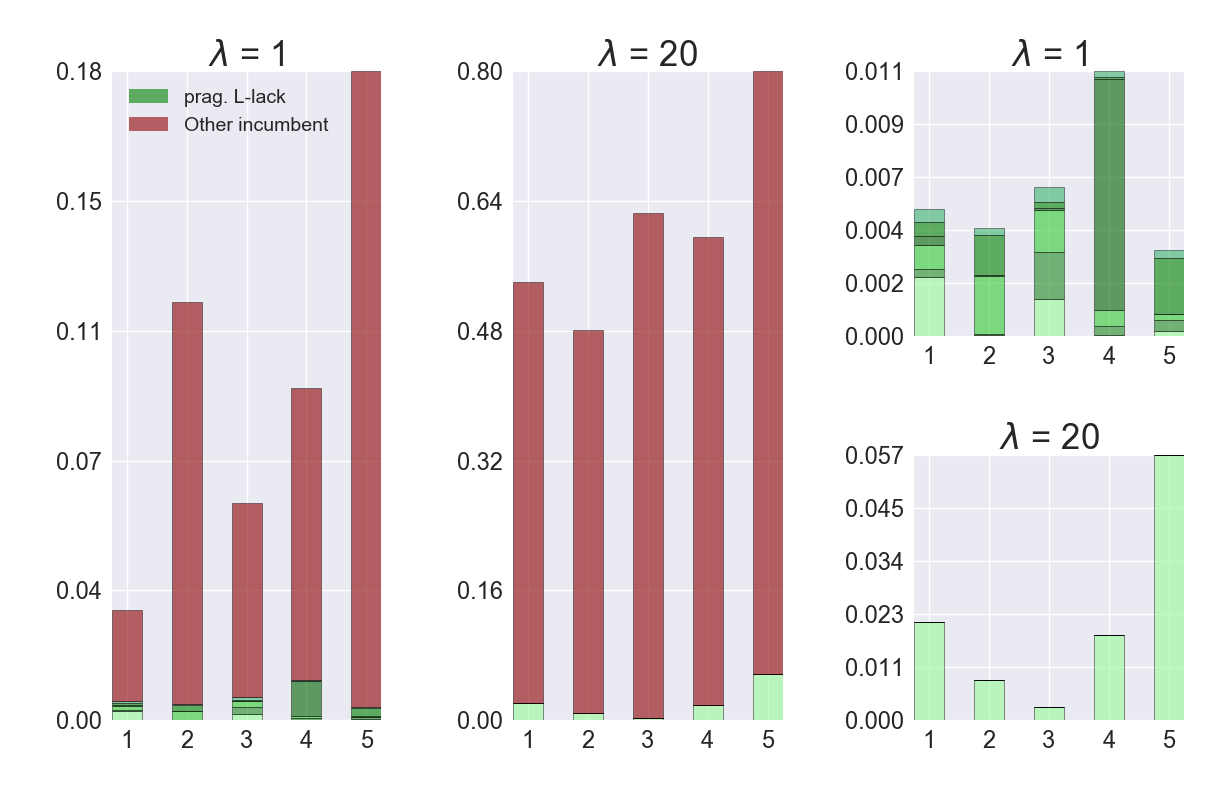
\includegraphics[width=\textwidth,height=8cm, keepaspectratio]{./plots/fig1-onlyr}
\caption{Stacked proportion of pragmatic $\Llack$-style types and majority types, when other
  than pragmatic $\Llack$, in $5$ independent populations after $50$ generations under only a
  pressure for communicative success. The right-most plots zoom in on only the proportion of target types. \tb{change plot to maj. type}}
\label{fig:only-R}
\end{figure}

As expected, selection based on communicative success is sensitive to $\lambda$ as it
influences signaling behavior, which in turn determines communicative success. This is
showcased in Figure \ref{fig:only-R}, which depicts the proportion of target types in $5$
independent populations after $50$ replicator steps. The plot also shows the proportion of the
\emph{majority type}, i.e., the type with the highest proportion in the final population. With
low $\lambda$ many types have very similar behavior, so that evolutionary selection lacks grip
and becomes very slow. The result is a very long transition with near stagnancy in a rather
homogeneous population with many types. Conversely, higher $\lambda$ promotes more rational
linguistic behavior, widening the gap in expressivity between types and promoting more
homogeneous populations. As suggested by Figure \ref{fig:only-R}, the majority in most
populations is not one of the six pragmatic $\Llack$-style types. That is, a pressure only for
communicative success does not lead to a prevalence of target types under any $\lambda$-value. For
instance, with $\lambda = 20$ $1000$ independent populations only had $11$ cases in which
the target type was the majority type, corresponding to a mean proportion of $0.003$ across
populations. By contrast, in $913$ cases the majority types had $\Lbound$ with close to an even
share between literal ($454$) and pragmatic types ($459$), corresponding to a mean proportion
of about $.48$ taken together.


\subsubsection{Iterated learning only}

\begin{figure}[t]
\centering
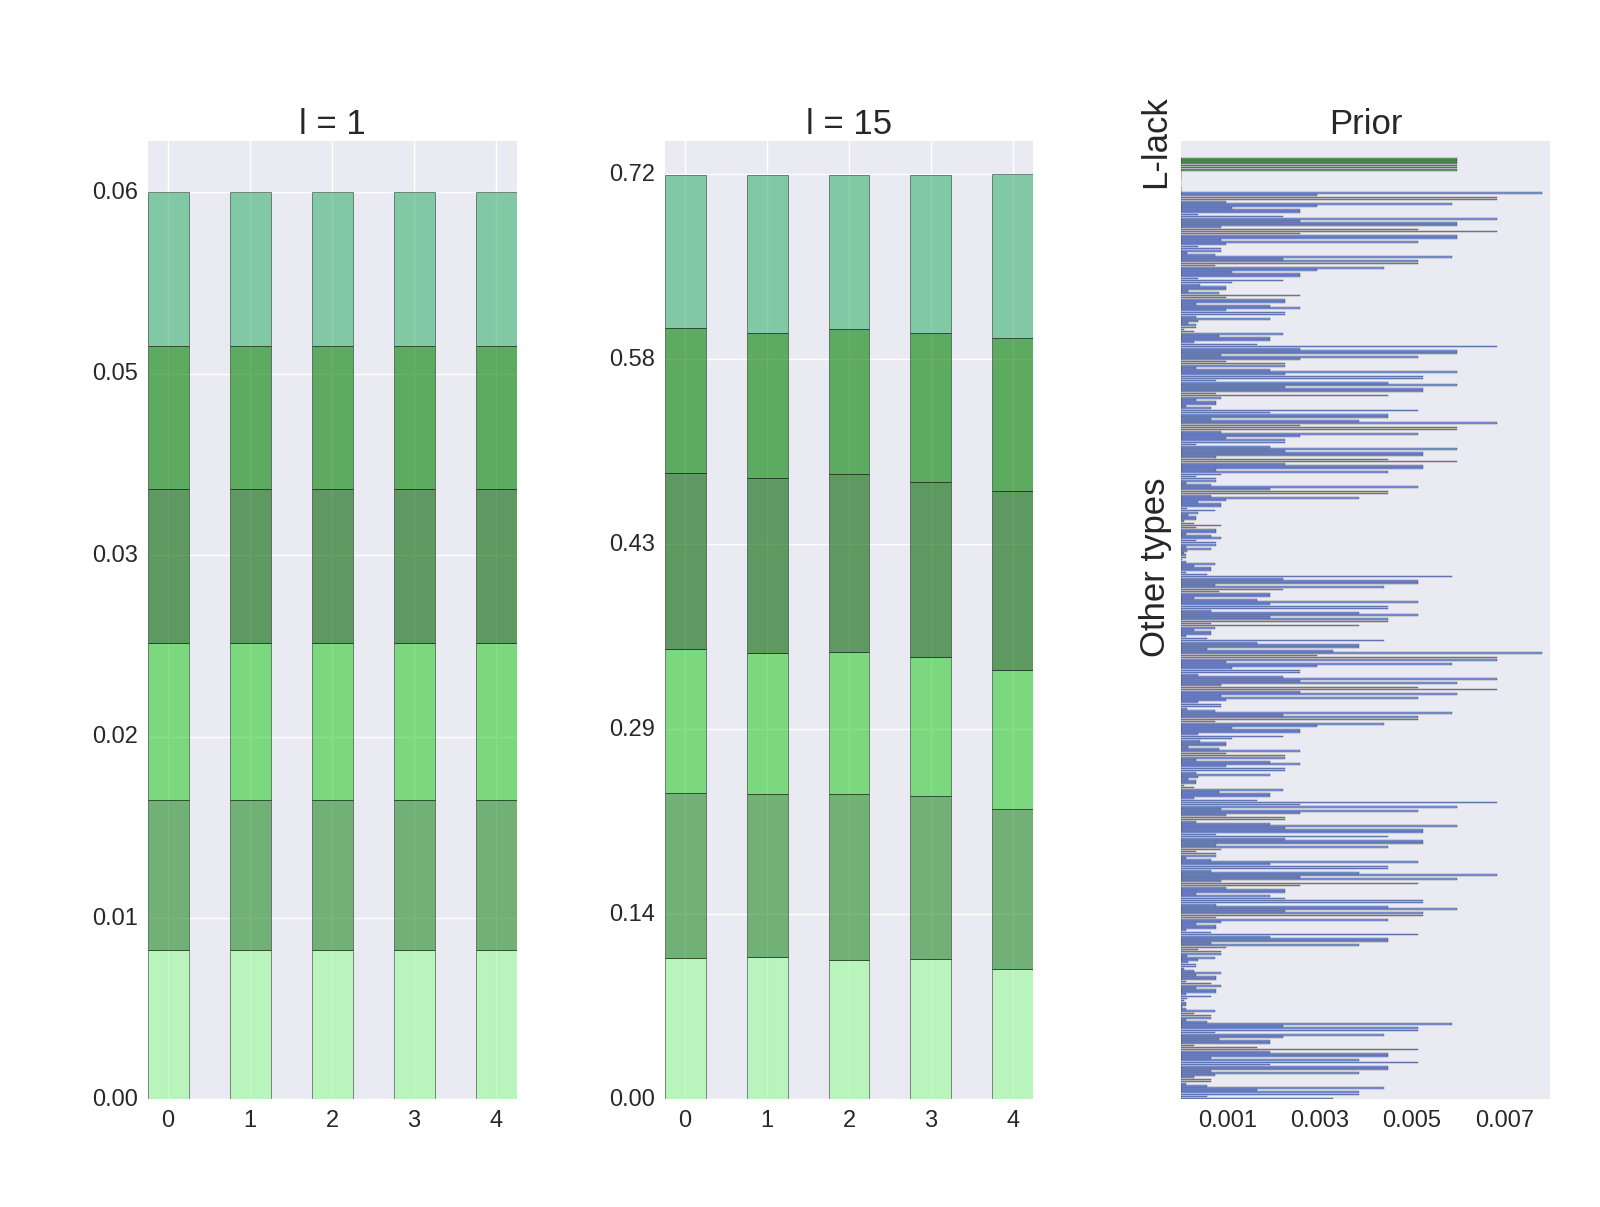
\includegraphics[width=1\textwidth,height=8cm,keepaspectratio]{./plots/fig2-onlym-pr}
\caption{Stacked proportion of pragmatic $\Llack$-style types and majority types, when other
  than pragmatic $\Llack$, in $5$ independent populations after $50$ generations under only a
  pressure for learnability ($\lambda = 20, k = 5$). The types' prior probability is shown in
  the right-most plot. \mf{explain the topmost part of the right plot?!} \tb{and change to maj. type in plot}}
\label{fig:only-M}
\end{figure}

The effect of iterated learning without a pressure for communicative success using either posterior
sampling ($l = 1$) or a stronger tendency towards posterior maximization ($l = 15$) is shown in
Figure \ref{fig:only-M} together with the prior over types. The prior shows that while users of
$\Llack$ are not the most favored by the inductive bias (compared, e.g., to $\Lall$) they are
nevertheless more advantaged than others, such as $\Lbound$, in virtue of the relatively simple
semantics they conventionalize (see Section~\ref{sec:an-induct-learn}). Crucially, $\Llack$
enables its users to convey each state with a single message when combined with pragmatic
reasoning provided sufficiently high $\lambda$. This makes it less likely to be confused with
other types if the learning data is not too sparse ($k \geq 5$). Put differently, learners have
a higher propensity to infer pragmatic $\Llack$ when the teacher's type produces very similar
data, such as when using $\Lbound$. Moreover, $\Llack$ is also less likely to be confused with
types with different observable behavior because its pragmatic use approximates a one-to-one
form-meaning mapping. As a consequence, a stronger propensity to maximize the posterior
increases their proportion in the population.

However, in contrast to a pressure only for communicative success with high $\lambda$ (see
Figure~\ref{fig:only-R}), learnability alone does not succeed in selecting for a single
prevalent type. Indeed, all six target types tend to coexist at roughly equal proportion. Each
is passed on to the next generation with the same faithfulness and, differently from a pressure
for communicative success, they do not stand in competition with each other. In $1000$
independent populations with $\lambda = 20$ all majority types were target types,
with each reaching approximately the same proportion of users in the population. As
with a pressure only for communicative success, low values of $\lambda$ make the differences in observable behavior
across types less pronounced and therefore reflect the learners' inductive bias more
faithfully, favoring functionally deficient but a priori preferred types such as those that use
$\Lall$. A pressure for learnability alone may consequently lead to a spread of communicatively
suboptimal types that are easier to learn. In the extreme, when $l = 1$ and $\lambda = 1$ all
of $1000$ independent populations had users of $\Lall$ as majority types.

\subsubsection{Combining pressures of communicative success and learnability}

Pressures for communicative success or learnability are not sufficient on their own to have a
single target type dominate the population. When pressured for communicative success, the slight
communicative advantage of $\Lbound$ users leads to the its prevalence. When pressured for
learnability, pragmatic $\Llack$ is promoted over functionally similar but semantically more
complex alternatives such as $\Lbound$. However, learnability alone does not foment the
propagation of a single target type across the population.

\begin{figure}[t]
\centering
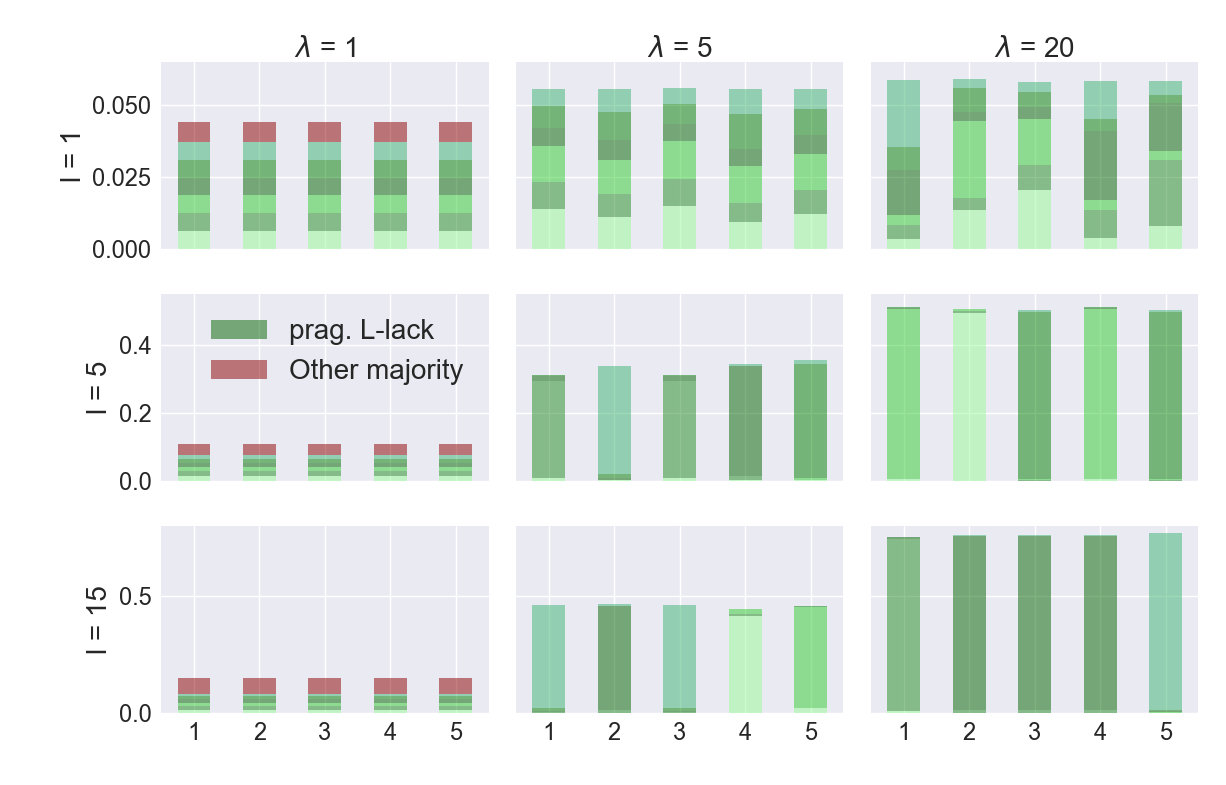
\includegraphics[width=1\textwidth,height=8cm,keepaspectratio]{./plots/fig3-r+m}
\caption{Stacked proportion of pragmatic $\Llack$-style types and majority types, when other than pragmatic $\Llack$, in $5$ independent populations after $50$ generations under both pressures ($k = 5$). \tb{change plot to maj. types}}
\label{fig:rmd}
\end{figure}

Figure \ref{fig:rmd} illustrates the combined effects of both pressures for a sample of
$\lambda$ and $l$ values. These results show that an inductive learning bias for simpler
semantics in tandem with functional pressure can lead to the selection of a single target
type. The proportion of a single majority target type increases with $\lambda$ and
$l$. Pressure for communicative success magnifies the effects of iterated learning and dampens
the proliferation of types of a kind that are equal in expressivity {\em and} learnability. A
pressure towards learnability favors the transmission of simpler semantics and thereby selects
for pragmatic language use.

As before, low $\lambda$ and $l$ lead to the prevalence of communicatively suboptimal types
that are a priori favored, such as $\Lall$. An increase in $\lambda$ leads to the selection of
target types but does not lead to monomorphic populations if learners sample from the
posterior. Finally, a combination of high $\lambda$ and $l$ leads to increasing proportions of
a single majority target type. The difference between the mean of the highest pragmatic
$\Llack$-like type in $1000$ independent populations and the highest proportion of other types
across $\lambda$ and $l$ values is shown in Figure \ref{fig:diff}.

\begin{figure}[t]
\centering
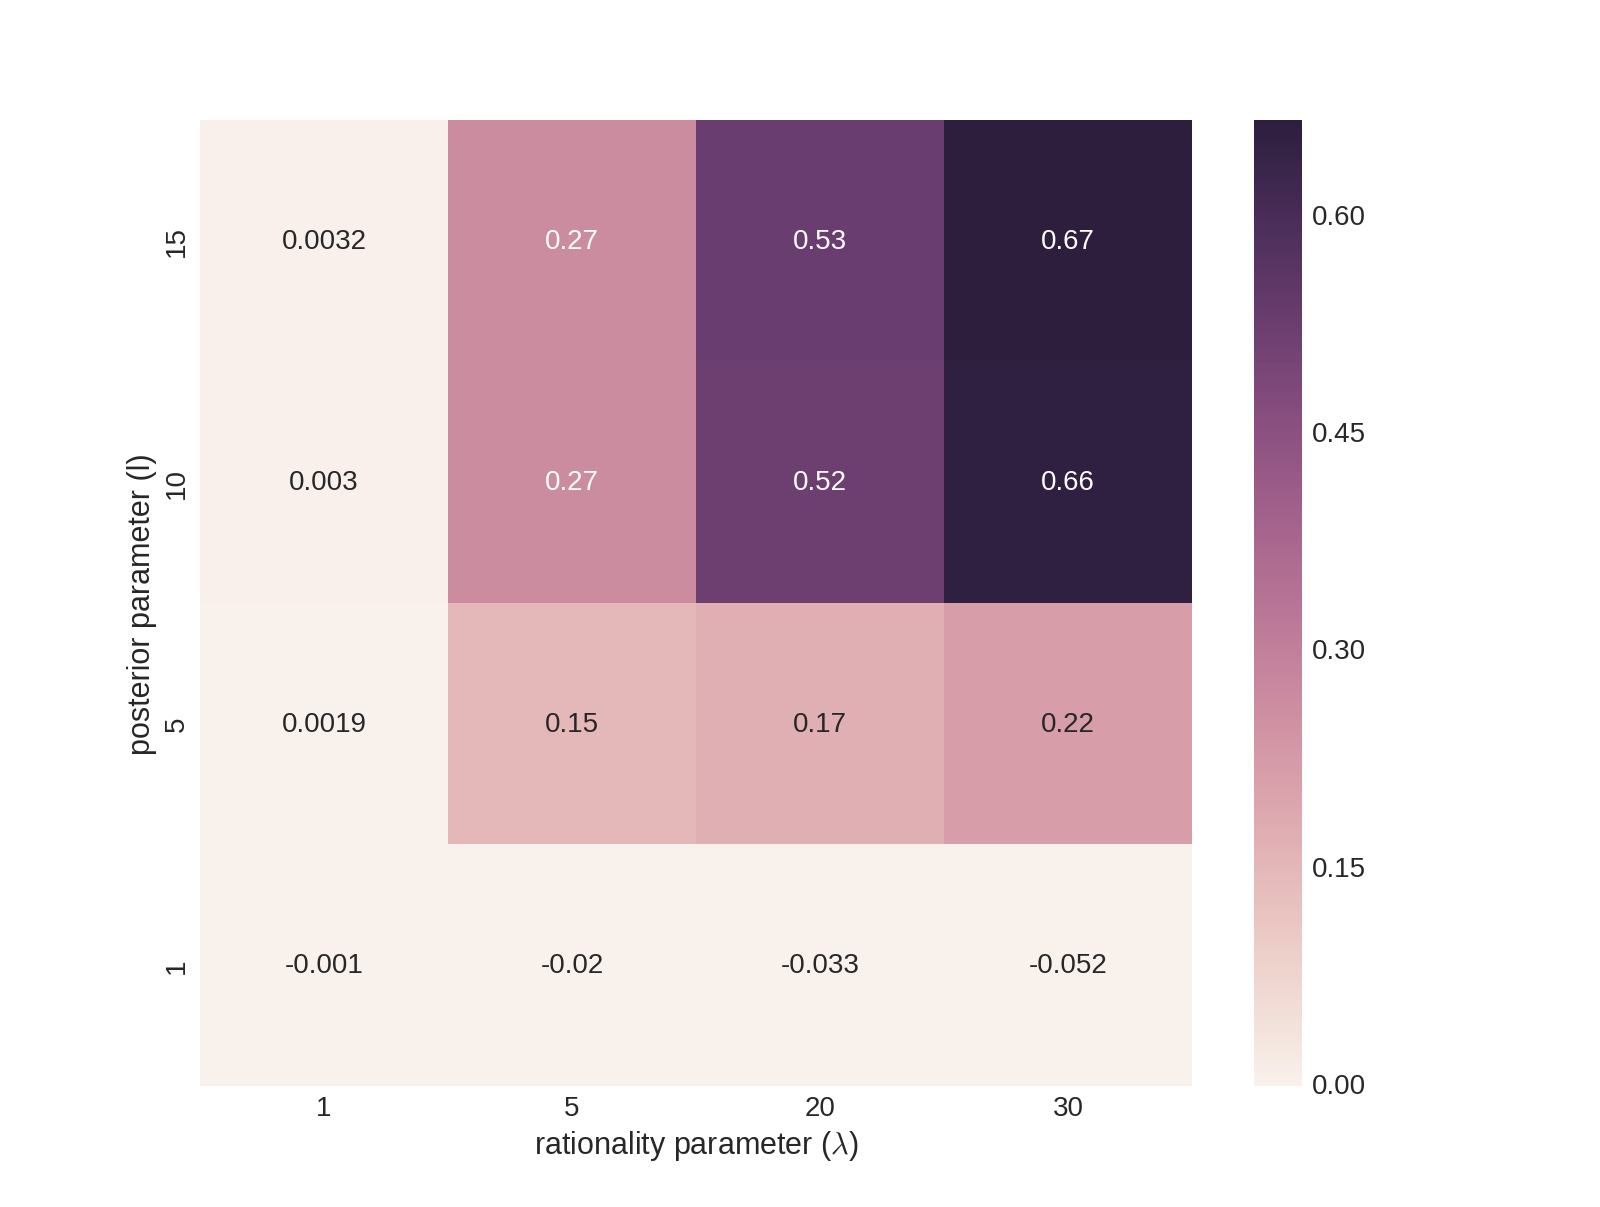
\includegraphics[width=1\textwidth,height=10cm,keepaspectratio]{./plots/fig4-incumbents-difference}
\caption{Difference between mean proportion of highest pragmatic $\Llack$ type and highest
  other type in $1000$ independent populations after $50$ generations under both pressures ($k
  = 5$).  \mf{the coloring is not that
    easy to decipher here; would a two-dimensional surface be possible and look better?}}
\label{fig:diff}
\end{figure}

As for the effect of the sequence length $k$ not mentioned so far, it influences populations in
a predictable way: small values lead to more heterogeneous populations that reflect the
learner's prior more faithfully. This is due to the fact that the likelihood that a small
sequence was produced by any type is relatively uniform (modulo prior). By contrast, larger
values increasingly allow learners to differentiate types with different signaling behaviors.

To recapitulate, other than the involvement of pressure on both communicative success and learnability,
the resulting proportion of pragmatic $\Llack$ speakers primarily hinges on three
factors. First, the degree, captured by $\lambda$, to which agents try to maximize
communicative success from their own subjective point of view. Second, the inductive bias,
which leads learners to prefer simpler over more complex semantic representations in
acquisition. Lastly, the learning behavior, captured by parameter $l$, where approximating a
MAP strategy magnifies the effects of the learning bias in tandem with replication.

In summary, target types, which represent the majority view of scalar implicatures, can come to
dominate the population if three assumptions are met: (i) language is pressured toward both
communicative success and learnability; (ii) pragmatic language use is an option; (iii) learners prefer
simpler over more complex lexical representations and exhibit a tendency towards the
acquisition of the type that best explains the learning data.


\section{General discussion}\label{sec:discussion}

The approach introduced here combines game theoretic models of functional pressure towards
efficient communication \citep{nowak+krakauer:1999}, effects of transmission perturbations on
(iterated) language learning \citep{griffiths+kalish:2007}, probabilistic speaker and listener
types of varied degrees of pragmatic sophistication \citep{frank+goodman:2012,
  franke+jaeger:2014} as well as reasoning about unobservable lexical representations
\citep{bergen+etal:2012,bergen+etal:2016}. This allows a conceptual investigation of the
co-evolution of conventional meaning and pragmatic language use. Main contributions of the
model are (i) its modular separation of communicative success and learnability on evolutionary
trajectories, (ii) the characterization of language learning as a joint inference over
pragmatic behavior and lexical meaning, and (iii) the possibility to trace the co-evolution of
conventional semantics and pragmatic use.

With respect to (i), \citet{kirby+etal:2015} propose a comparable model of the interaction
between a lexicon's expressivity and its learnability. One of its main differences to our proposal lies in 
the former force exerting pressure only in the production of learning data. The pressure towards communicative success 
within a population central to replication is absent. Put differently, we consider a pressure for mutual understanding 
that may indirectly select for expressive types, i.e., those that can convey states unequivocally, whereas Kirby et al. only
consider the bearing that the latter ability has on the production of learnable data. We see two main reasons
for considering communicative success rather than expressivity, and to only considering it in learning. First, learnability alone can 
lead to the acquisition of functionally defective languages, as showcased by $\Lall$ (cf. \citealt{kirby+etal:2008,silvey+etal:2014}, and \citealt{fay+etal:2013} for review of laboratory results). Second and more importantly, types may be equally expressive but their performance as means of information transfer crucially depends not only on themselves but on the population they find themselves in (cf. the competition of types of a kind in Figure \ref{fig:rmd} and their lack of competition in Figure \ref{fig:only-M}). That is, we contend that having an expressive lexicon that generates learnable data does not  in itself capture a type's arguably central communicative function of transferring information to peers. Under this view, a type's expressiveness is secondary to its ability to communicative successfully. Acquiring a maximally expressive type is of little use when it is not understood in its population. 

The main result of our case study is that types that correspond to the majority view of scalar
implicatures (scalar readings are non-lexicalized pragmatic enrichments) can come to dominate a
population. This can happen under the assumption that simpler semantic representations are more
likely to be learned (cf. \citealt{chater+vitanyi:2003}). Pragmatic language use can be
recruited indirectly by a preference for simpler lexical concepts. Under this view, semantics
and pragmatics play a synergic role: pragmatic use allows maintenance of simpler concepts;
pressure towards representational simplicity indirectly promotes pragmatic over literal
language use. As a consequence, iterated transmission and use of language lead to a
regularization that may explain the lack of lexicalization of systematic pragmatic enrichments.

While the results of this case study are interesting, they also raise a number of critical
issues. First of all, while many favorable parameter settings exist which lead to a prevalence
of target types, other types are usually represented in non-negligible proportions. This may
just be a technical quirk of the mutator step. But there is a related issue of empirical
importance. Several experimental studies on scalar implicatures suggest that participants can
be classified as either semantic or pragmatic users of, in particular, \emph{some}
\citep[e.g.][]{BottNoveck2004:Some-Utterances,NieuwlandDitman2010:On-the-incremen,DegenTanenhaus2012:Processing-Scal}. The
former consistently accept \emph{some} where \emph{all} would be true as well, the latter do
not. Interestingly, in our simulations when a target type is the majority type an inflated
proportion of the population uses compatible lexica with a lexicalized upper bound. Particularly in those parameter
settings where the prior influences the outcome less. In other words, we do find a tendency toward a similar co-existence
of semantic and pragmatic types. Whether this analogy has any further explanatory value is an interesting path for future
exploration. \tb{I some qualifications. While it is indeed true that $\Lbound$'s proportion is inflated relative to other types in the hypothesis space, it is never the second most prolific type (which is what the above hopefully is not taken to suggest, otherwise it should be changed). As is to be expected, $\Lbound$ fares best when $l$ is low and $\lambda$ is high. Even then, it usually ranks around $5$-th with a mean proportion of its kind of about $0.01 - 0.05$. As $l$ increases, it gets pushed back. Second or third place are usually instead literal $\Llack$ or types that lexicalize ``all'', ``not all'' and ``none''. In short; yes, there is a inflated proportion but only compared to the whole population. Other particular types are usually more prolific. This is very likely due to the strong prior disadvantage of $\Llack$. In light of this I'm uncertain whether we want to keep this paragraph as is. I tend towards `yes' but let me know if you think otherwise.}

Another important issue that is not addressed in the model are potential costs associated with
pragmatic reasoning. Here, we simply assumed that literal and pragmatic reasoning strategies
exist from the start and are equally costly to apply. In contrast, empirical results suggest
that the computation of a scalar implicature may involve additional cognitive effort
\citep[e.g.][]{BrehenyKatsos2006:Are-Generalised,deNeys+schaeken:2007,huang+snedeker:2009,Jr.Bailey2013:Possibly-all-of}. Extensions
of the model presented here to include processing costs for pragmatic language use would be
interesting future work. It seems plausible that effects of reasoning cost may trade off with
the frequency with which a given scalar expression is used. It may be that frequently drawn
scalar implicatures lexicalize to avoid cost, whereas infrequent ones are derived on-line to
avoid more complex lexical concepts during acquisition. Such a prediction would lend itself to
empirical testing in line with a recent interest in differences between various scalar
implicature triggers \citep{Tielvan-TielMiltenburgvan-Miltenburg2014:Scalar-Diversit}.


Our case study could be criticized as follows: all it shows is that scalar implicatures do not
lexicalize because upper bounds are dispreferred concepts. This criticism would be too
superficial and highly unjust. Dispreferred lexical concepts can thrive under evolutionary
selection. Lexicalized upper-bounds can dominate a population because they may boost
communicative efficiency. But they do not have to. Moreover, even without selective pressure
for communicative efficiency, it is not the case that necessarily the types that are most
likely \emph{a priori} will dominate. The dynamics of iterated learning are not that
trivial. Iterated learning does not necessarily promote the \emph{a priori} more likely type,
but tends to promote a type $t$ based on a gradient of how many other types might likely mutate
into $t$, so to speak. Taken together, without an explicit model of the interaction between
pressure for efficiency and learnability, it is far from trivial to judge whether or when
preferred or dispreferred concepts can be adaptive. This is why a major contribution of this
paper is the arrangement of many different ingredients into a joined model of the co-evolution
of lexical meaning and pragmatic use. 

What is more, it is not that we just assumed a prior disadvantage of lexicalized upper
bounds. We tried to motivate and formalize a general assumption about concepts' complexity
with a concrete, albeit provisional proposal. The specification of a learning bias in terms of
a ``grammar of concepts'' can and should be seen critically, however. Much depends on the
primitives of such a grammar. For instance, the concept ``none or all'' is the most complex in
Table~\ref{tab:concepts}. But consider adding a primitive operation on sets $A \smile B$
which is true if and only if $\neg(A \cap B \neq \emptyset \wedge A \neq \emptyset)$. The
concept ``none or all'' would then be one of the simplest. Clearly, further research, empirical
and conceptual, into the role of representational complexity, processing costs and learning
biases is needed. The model here makes a clear and important contribution nonetheless: it shows
how simplicity of concepts can interact with use and evolutionary selection to show that
without pragmatic language users we would not see simpler concepts emerge in what may be a
natural way. Future work should also include the possibility that conceptual simplicity may
itself be a notion that is subject to evolutionary pressure
\citep[cf.][]{ThompsonKirby2016:Culture-Shapes-}. 

Finally, our case study should not be interpreted as a proposal for a definite explanation of
how scalar implicatures evolved. Other factors should be considered eventually even if they
will lead to much more complex modeling. One such factor is the observation that
non-lexicalized upper bounds allow a broader range of applicability, e.g., when the speaker is
not certain as to whether \emph{all} is true. This may suggest an alternative argument for why
upper-bounded meanings do not conventionalize based on functional criteria only: should
contextual cues provide enough information to the hearer to identify whether a bound is
intended to be conveyed pragmatically, then this is preferred over expressing it overtly
through longer expressions, e.g., by saying {\em some but not all} explicitly. Importantly,
although morphosyntactic disambiguation may be dispreferred due to its relative length and
complexity \citep{piantadosi+etal:2012b}, it allows speakers to enforce an upper-bound and
override contextual cues that might otherwise mislead the hearer. In a nutshell, this
explanation posits that scalar implicatures fail to lexicalize because, all else being equal,
speakers prefer to communicate as economically as possible and pragmatic reasoning enables them
to do so. What this alternative explanation does not explain is why functional pressure does
not lead to the emergence of different, equally costly lexical items to express different
knowledge states of the speaker. Looking at pressure from learnability might come in again. The
present work made a first start and gave a framework for exploring exactly these issues
systematically.

\section{Conclusion}
The cultural evolution of meaning is influenced by intertwined pressures. We set out to
investigate this process by putting forward a model that combines a pressure toward successful
information transfer with perturbations that may arise in the transmission of linguistic
knowledge in acquisition. Its objects of selection and replication are pairs of lexical
meanings and patterns of language use. This allows the model to trace the interaction between
conventional meaning and pragmatic use. Additionally, it takes the challenge serious of neither
semantics nor pragmatics being directly observable. Instead, learners need to infer these
unobservables from overt data that results from their combination.  These components and their
mutual influence were highlighted in a case study on the lack of lexical upper-bounds in weak
scalar expressions that showed that, when pressured for learnability and communicative success, the
former force drives for simpler semantic representations inasmuch as pragmatics can compensate
for lack of expressivity in use. That is, the relative learning advantage of simpler semantics
in combination with functional pressure in use may offer an answer to why natural languages
fail to lexicalize systematic pragmatic inferences. And, more broadly, to a division of labor
between semantics and pragmatics.

\bibliographystyle{chicago}
\bibliography{./bounds-rmd}

\newpage

\appendix


\section{notes}

\begin{itemize}
\item \mf{The text frequently uses the term ``expressivity'' and ``pressure for/towards
    expressivity''. I have mixed feelings about this. First of all, I don't know what
    ``expressivity'' really is. It seems to relate to a lexicon: how much information can the
    lexicon convey about the states. But we do not model selection of expressivity, but
    selection of communicative success relative to the population state. The difference is very
    pronounced: there can be several maximally expressive lexica with huge differences in their
    communicatively success or expected utility for a given population state. We only
    indirectly select for expressivity, and we don't necessarily select for expressivity of a
    lexicon. \dots It may be that ``expressivity'' is very much Edinburgh terminology where
    exactly the picture of communication success in the current population is missing. I might
    be wrong though. Possibly, we should introduce this distinction (with this terminology) and
    use it also in the general discussion to relate our work to those articles from the
    iterated-learning community that bring in some pressure for ``expressivity'' but not
    communicative efficiency (if that is what they do, I don't know?).}
\end{itemize}


\end{document}
